\documentclass[aspectratio=169]{beamer}
\PassOptionsToPackage{english}{babel}
\usepackage{standardslides}

\usepackage{svg}

\usepackage{tikz}
\usepackage{pifont}
\usepackage{listings}
\usepackage{colortbl}
\newlength{\listingframemargin}
\setlength{\listingframemargin}{1em}
\newlength{\listingmargin}
\setlength{\listingmargin}{0.08\textwidth}

\definecolor{codeDarkGray}{gray}{0.2}
\definecolor{codeGray}{gray}{0.4}
\definecolor{codeLightGray}{rgb}{0.94,0.94,0.91}
\definecolor{codeBorder}{rgb}{0.34,0.24,0.21}
\definecolor{MidnightBlue}{rgb}{0.1, 0.1, 0.8}

\lstdefinestyle{standard}{%
  belowcaptionskip=0.5\baselineskip,
  breaklines=true,
  frameround=tttt,
  % frame=false,
  xleftmargin=0em,
  xrightmargin=0em,
  showstringspaces=false,
  showtabs=false,
  % tab=\smash{\rule[-.2\baselineskip]{.4pt}{\baselineskip}\kern.5em},
  basicstyle= \fontfamily{pcr}\selectfont\tiny\bfseries,
  keywordstyle= \bfseries\color{MidnightBlue}, %\color{codeDarkGray},
  commentstyle= \itshape\color{codeGray},
  identifierstyle=\color{codeDarkGray},
  stringstyle=\color{BurntOrange}, %\color{codeDarkGray},
  numberstyle=\tiny\ttfamily,
  % numbers=left,
  numbersep = 1em,
  % stepnumber = 1,
  % captionpos=t,
  tabsize=2,
  % backgroundcolor=\color{codebLightGray},
  rulecolor=\color{codeBorder},
  framexleftmargin=\listingframemargin,
  framexrightmargin=\listingframemargin
}

\newcommand{\inputCodeBlock}[1]{%
  % \begin{mybox}
    \begin{center}
      % \begin{minipage}[c]{0.7\textwidth}
        \lstinputlisting[%
          style = standard,
          language = c++,
          morekeywords={constexpr,noexcept,decltype,size_t,uint32_t,uint64_t,__m256i,__m256,__m256d,__m128i,__m128,__m128d}
        ]{#1}
      % \end{minipage}
    \end{center}
  % \end{mybox}
}

\def\UrlBigBreaks{\do\/\do-\do:}

\title{%
  Illustrative Visualization: Photic Extremum Lines%
}
% \subtitle{Master's Thesis Defense and Presentation}
\author{Markus Pawellek}

\bibliography{references}

\begin{document}

\selectlanguage{english}

{ % all template changes are local to this group.
  \setbeamertemplate{navigation symbols}{}
  \begin{frame}<article:0>[plain]
    % \begin{tikzpicture}[remember picture,overlay]
    %   \node[at=(current page.center)] {
    %     \includegraphics[keepaspectratio,
    %                      width=1.2\paperwidth,
    %                      height=\paperheight]{images/banner.png}
    %   };
    % \end{tikzpicture}
    \center
    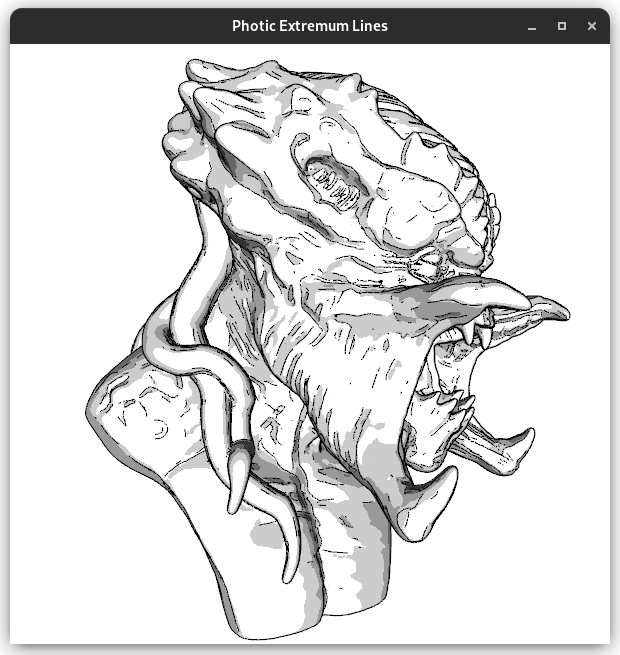
\includegraphics[width=0.49\textwidth,trim={15px 15 15 50},clip]{images/predator-intro.png}
    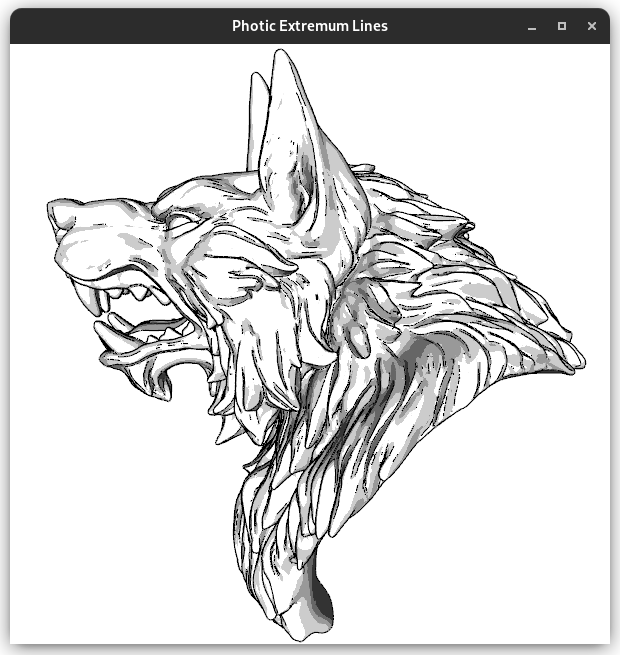
\includegraphics[width=0.49\textwidth,trim={15px 15 15 50},clip]{images/werewolf-intro.png}
  \end{frame}
}

\setbeamertemplate{background}{
  
\includegraphics[width=\paperwidth,height=\paperheight]{images/background-luyu.png}
}

\frame{\titlepage}
\begin{frame}{Outline}
  \footnotesize
  \hfill\parbox[t][7cm][l]{0.9\textwidth}{\tableofcontents}
\end{frame}

\section{Related Work}
  \begin{frame}{Related Work}
    \small
    \onslide<+->
    \textbf{Tools}
    \begin{description}
      \item<+->[\citeyear{isenberg2003}] \citeauthor{isenberg2003} \citetitle{isenberg2003}
      \item<+->[\citeyear{rusinkiewicz2004}] \citeauthor{rusinkiewicz2004} \citetitle{rusinkiewicz2004}
    \end{description}
    \onslide<+->
    \textbf{Algorithm}
    \begin{description}
      \item<+->[\citeyear{xie2007}] \citeauthor{xie2007} \citetitle{xie2007}
      \item<+->[\citeyear{zhang2010}] \citeauthor{zhang2010} \citetitle{zhang2010}
    \end{description}
  \end{frame}

\section{Mathematical Preliminaries}
  \begin{frame}{Mathematical Preliminaries: %
    \only<1-3>{Mesh Function}%
    \only<4-7>{Mesh Function Gradient}%
    \only<8>{Directional Derivatives}%
  }
    % \begin{description}
    %   \item[\citeyear{max1999}] \citeauthor{max1999} \citetitle{max1999}
    %   \item[\citeyear{rusinkiewicz2004}] \citeauthor{rusinkiewicz2004} \citetitle{rusinkiewicz2004}
    %   \item[\citeyear{meyer2001}] \citeauthor{meyer2001} \citetitle{meyer2001}
    % \end{description}
    \begin{figure}
      \center
      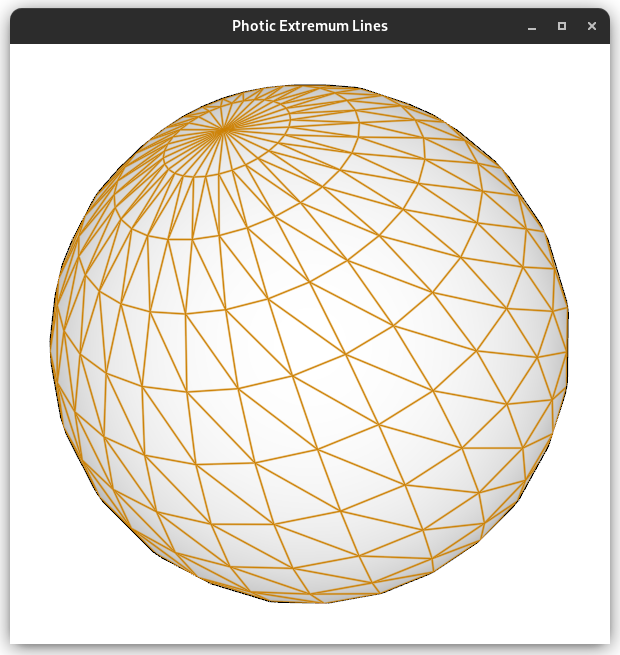
\includegraphics[height=0.45\textheight,trim={15px 15 15 50},clip]{images/sphere-wireframe.png}
      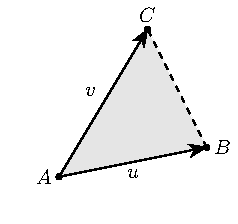
\includegraphics[height=0.45\textheight]{figures/triangle.pdf}
    \end{figure}
    \vfill
    \only<1-3>{%
      \begin{itemize}
        \item<2-> $\function{f}{S}{\setReal}$ on mesh $S$ characterized by its values at vertices
        \item<3-> For interiors of faces, use barycentric interpolation
      \end{itemize}
    }%
    \only<4-6>{%
      \begin{itemize}
        \item<5-> Compute $\nabla f$ for each face
        \item<6-> For each vertex, accumulate weighted and rotated \\
        gradients for adjacent faces
      \end{itemize}
    }%
    \only<7>{%
      \begin{mybox}
        \[
          \mathrm{I}_{uv} \define
          \begin{pmatrix}
            \norm{u}^2 & \scalarProduct{u}{v} \\
            \scalarProduct{u}{v} & \norm{v}^2
          \end{pmatrix}
          \separate
          \nabla f =
          \begin{pmatrix}
            u & v
          \end{pmatrix}
          \mathrm{I}_{uv}^{-1}
          \begin{pmatrix}
            f(B) - f(A) \\
            f(C) - f(A)
          \end{pmatrix}
        \]
      \end{mybox}
    }%
    \only<8>{%
      \begin{mybox}
        \[
          \partial_w f(x) = \scalarProduct{\nabla f(x)}{w}
          \separate
          \mathscr{D}_f\, g(x) \define \scalarProduct{\nabla g(x)}{\frac{\nabla f(x)}{\norm{\nabla f(x)}}}
        \]
      \end{mybox}
    }%
  \end{frame}

\section{Photic Extremum Lines}
  \begin{frame}{Photic Extremum Lines}
    \begin{minipage}[c]{0.4\textwidth}
      \center
      \only<1>{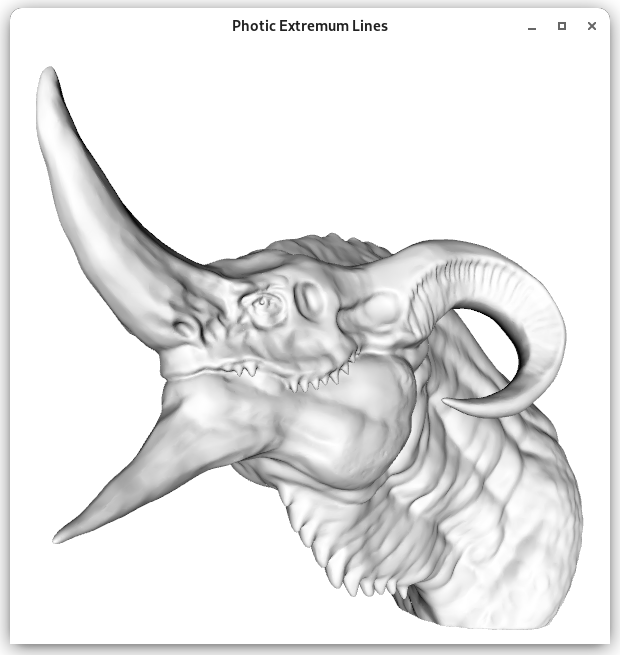
\includegraphics[width=\textwidth,trim={15px 15 15 50},clip]{images/dragon-head-vertex-lighting.png}}%
      \only<2-3>{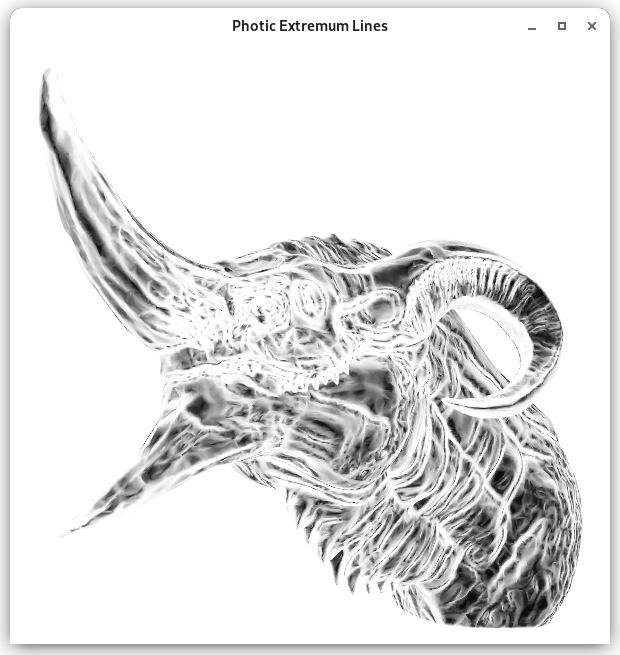
\includegraphics[width=\textwidth,trim={15px 15 15 50},clip]{images/dragon-head-light-variation.png}}%
      \only<4>{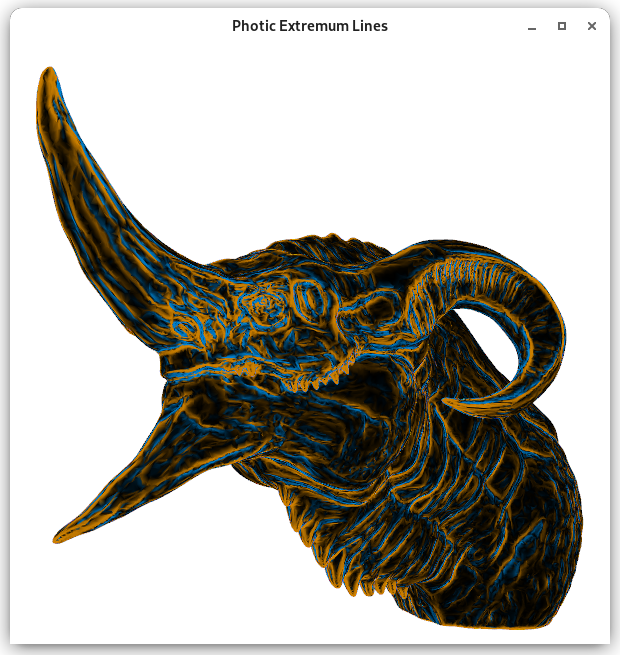
\includegraphics[width=\textwidth,trim={15px 15 15 50},clip]{images/dragon-head-light-variation-slope.png}}%
      \only<5>{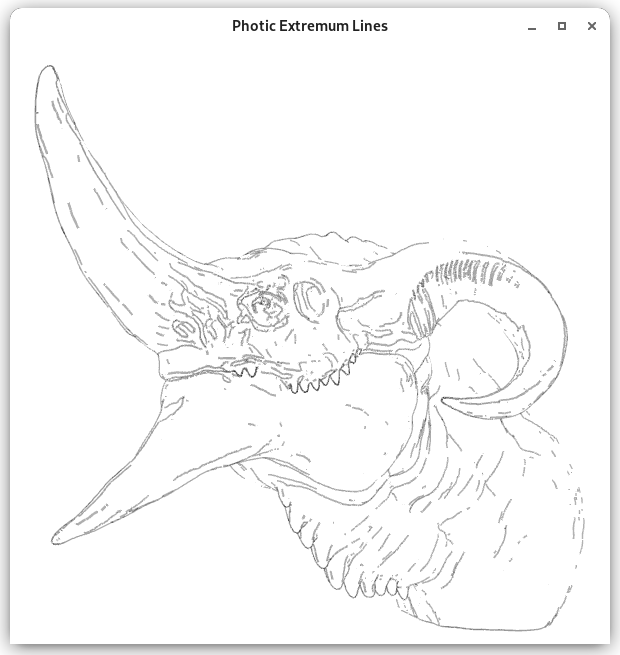
\includegraphics[width=\textwidth,trim={15px 15 15 50},clip]{images/dragon-head-pel-shader.png}}%
      \only<6>{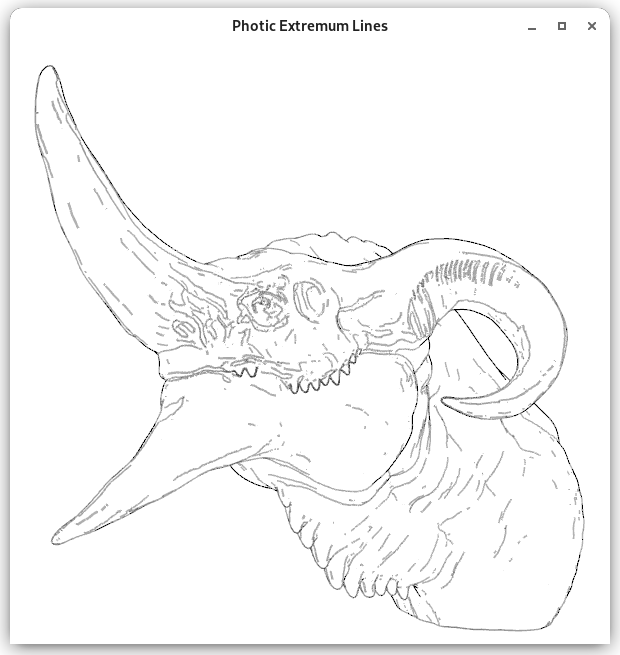
\includegraphics[width=\textwidth,trim={15px 15 15 50},clip]{images/dragon-head-contour-pel-shader.png}}%
      \only<7>{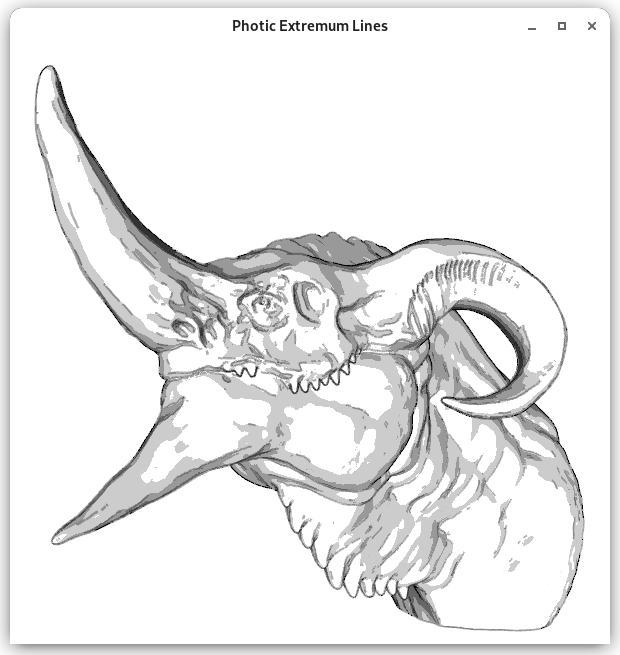
\includegraphics[width=\textwidth,trim={15px 15 15 50},clip]{images/dragon-head-contour-pel-toon-shader.png}}%
    \end{minipage}
    \hfill
    \begin{minipage}[c]{0.55\textwidth}
      \begin{itemize}
        \item<1-> Scalar illumination function \\
        $\function{\varphi}{S}{\setReal}$ on mesh $S$ \\
        (e.g. directional light source)
        \item<2-> Variation of illumination $\norm{\nabla\varphi}$
      \end{itemize}
      \onslide<3->
      \bigskip
      \begin{mybox}
        \textbf{Photic Extremum}\\
        Illumination variation in the direction \\
        its gradient reaches local maximum
        \onslide<4->
        \[
          \mathscr{D}_\varphi \norm{\nabla \varphi}(x) = 0
          \separate
          \mathscr{D}_\varphi^2 \norm{\nabla \varphi}(x) < 0
        \]
      \end{mybox}
    \end{minipage}
  \end{frame}

\section{Algorithm}
  \begin{frame}{Algorithm: Overview}
    \begin{mybox}
      \pause
      \begin{enumerate}
        \item<+-> Compute $\varphi$
        \item<+-> Compute $\frac{\nabla\varphi}{\norm{\nabla\varphi}}$ and $\norm{\nabla\varphi}$
        \item<+-> Compute $\mathscr{D}_\varphi \norm{\nabla\varphi}$
        \item<+-> Compute $\mathscr{D}^2_\varphi \norm{\nabla\varphi}$
        \item<+-> Detect line vertices on edges by testing for photic extremums
        \item<+-> Trace and filter out lines by using a threshold
        \item<+-> Render visible lines
      \end{enumerate}
    \end{mybox}
  \end{frame}

  \begin{frame}{Algorithm: Line Detection and Tracing}
    \begin{minipage}[c]{0.49\textwidth}
      \only<1-2>{%
      \begin{itemize}
        \item<1-> For each edge $[v,w]\subset S$, \\
          check zero-crossing:
          \[
            h(x) \define \mathscr{D}_\varphi \norm{\nabla\varphi}(x)
          \]
          \[
            h(v)h(w) < 0
          \]
        \item<2-> Approximate zero-crossing:
        \[
          p \define \frac{\absolute{h(w)}v + \absolute{h(v)}w}{\absolute{h(v)} + \absolute{h(w)}}
        \]
      \end{itemize}
      }%
      \only<3-4>{%
      \begin{itemize}
        \item<3-> Check maximum condition:
        \[
          \mathscr{D}_\varphi^2\norm{\nabla\varphi}(p) < 0
        \]
        \item<4-> For each triangle, connect \\
        valid zero-crossings of adjacent \\
        edges to segments
      \end{itemize}
      }%
      % For this we can use a geometry shader.
      % For every face, compute zero crossings at edges.
      % If point fulfills maximum condition, make it a line vertex.
      % Two line vertices are emitted as line segment.
    \end{minipage}
    \hfill
    \begin{minipage}[c]{0.49\textwidth}
      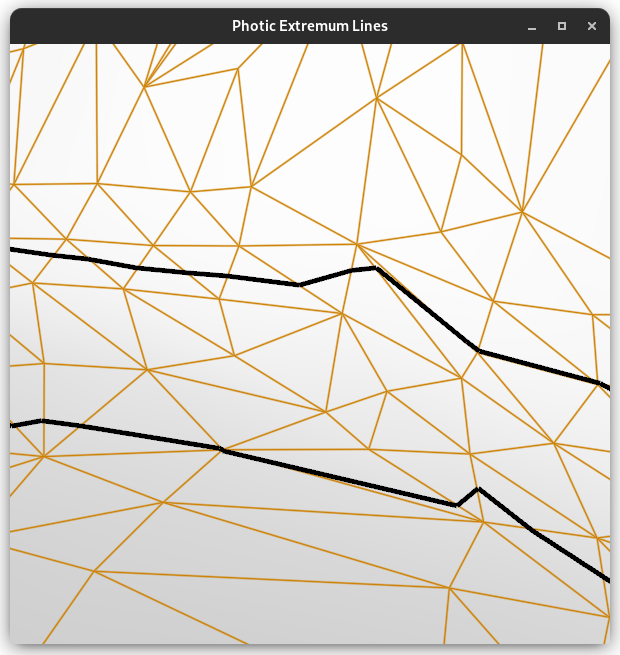
\includegraphics[width=0.9\textwidth,trim={15px 15 15 50},clip]{images/subpolygon-lines.png}
    \end{minipage}
  \end{frame}

  \begin{frame}{Algorithm: Threshold Filter}
    \begin{figure}
      \center
      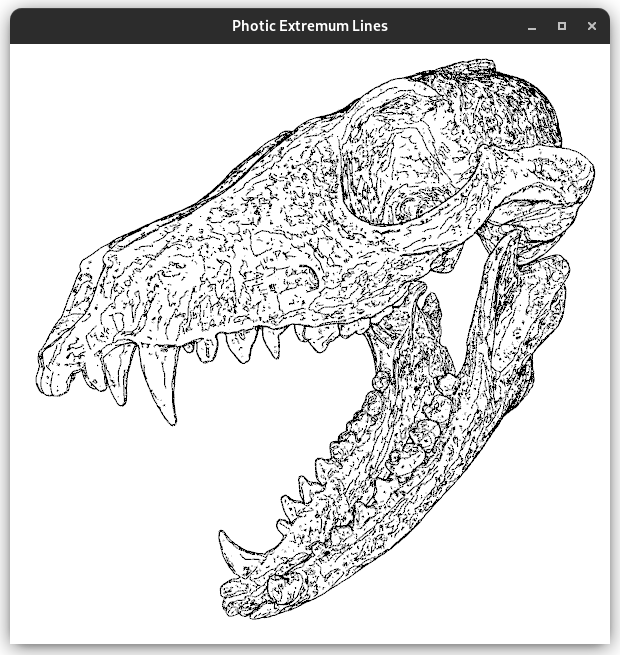
\includegraphics[height=0.49\textheight,trim={15px 15 15 50},clip]{images/fox-skull-threshold-low.png}
      \hspace{5em}
      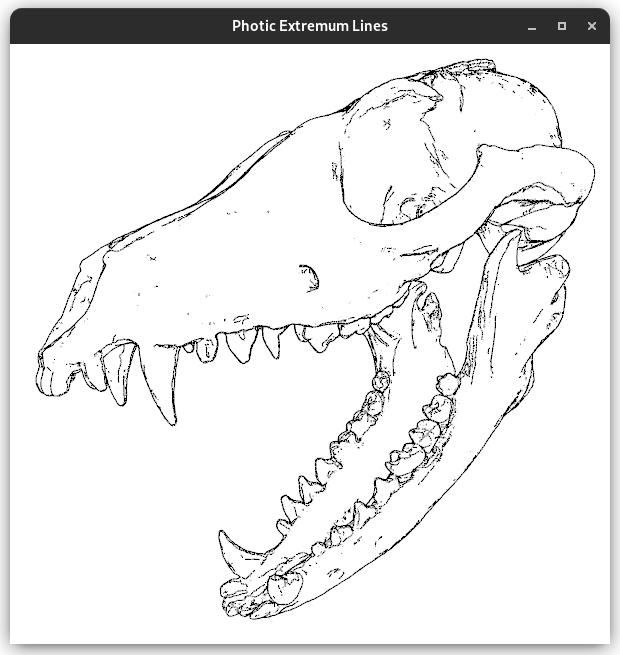
\includegraphics[height=0.49\textheight,trim={15px 15 15 50},clip]{images/fox-skull-threshold-mid.png}
    \end{figure}
    \pause
    Strength $S$ of photic extremum or strength $\mathscr{S}$ of photic extremum line $L$:
    \begin{mybox}
      \[
        S(x) = \norm{\nabla \varphi(x)} > T
        \qquad \text{or} \qquad
        \mathscr{S}(L) \define \integral{L}{}{\norm{\nabla \varphi(s)}}{s} > T
      \]
    \end{mybox}
  \end{frame}

  \begin{frame}{Algorithm: Hidden Line Removal}
    \begin{figure}
      \center
      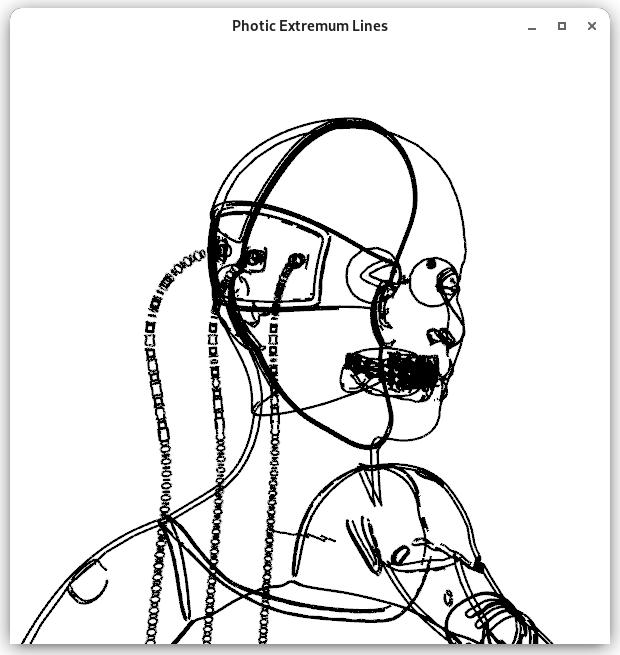
\includegraphics[height=0.49\textheight,trim={15px 15 15 50},clip]{images/cyborg-contour-pel-hidden-shader.png}
      \hspace{5em}
      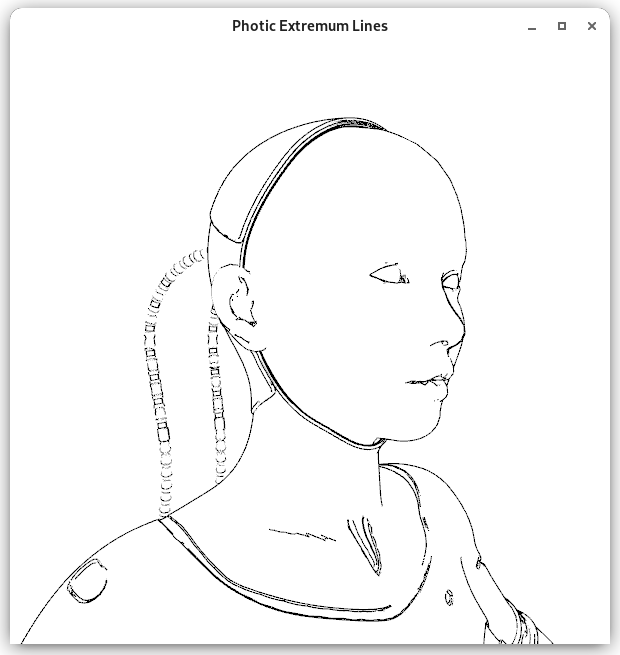
\includegraphics[height=0.49\textheight,trim={15px 15 15 50},clip]{images/cyborg-contour-pel-shader.png}
    \end{figure}
    \bigskip
    \pause
    \begin{itemize}
      \item<+-> Use z-buffer in a two-pass rendering approach
      \item<+-> Render the shape with a custom shader for its fragments
      \item<+-> Render visible feature lines by using depth testing
    \end{itemize}
  \end{frame}

\section{Results}
  \begin{frame}{Results: General Properties}
    \begin{minipage}[c]{0.49\textwidth}
      \center
      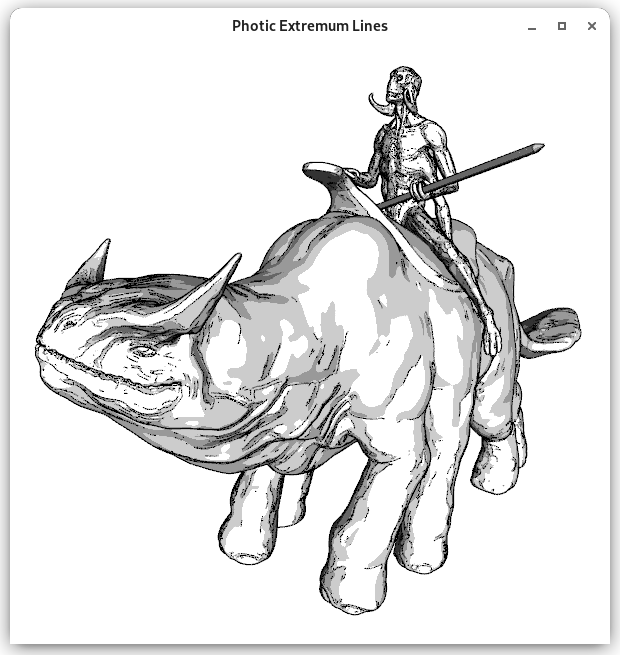
\includegraphics[width=\textwidth,trim={15px 15 15 50},clip]{images/rider.png}
    \end{minipage}
    \pause
    \begin{minipage}[c]{0.49\textwidth}
      \begin{itemize}
        \item<+-> Able to render convex and concave edges simultaneously
        % \item<+-> Convey shapes similar to human perception
        \item<+-> Applicable to isosurfaces of volumetric datasets
        \item<+-> Highly dependent on scalar illumination function
        \item<+-> Computationally expensive: \\
        interactive on CPU, \\
        real-time capable on GPU
      \end{itemize}
    \end{minipage}
  \end{frame}

  \begin{frame}{Results: Contours vs. Photic Extremum Lines}
    \begin{figure}
      \center
      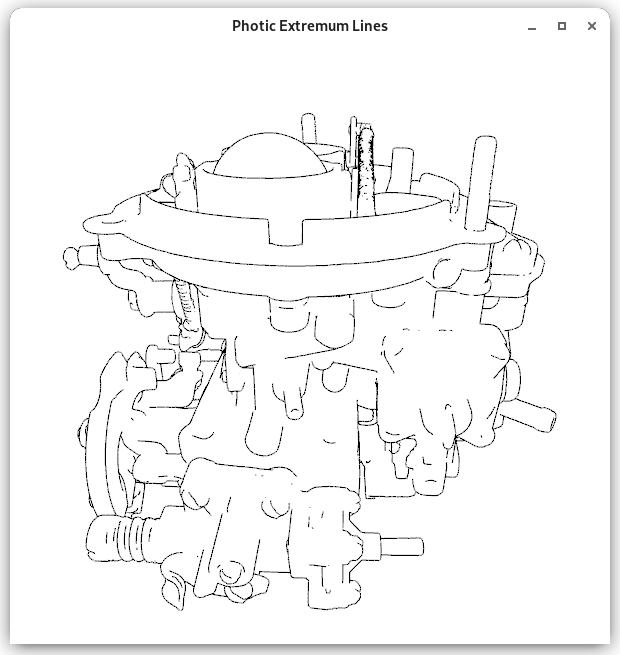
\includegraphics[height=0.49\textheight,trim={15px 15 15 50},clip]{images/tile-contour-shader.png}
      \hspace{5em}
      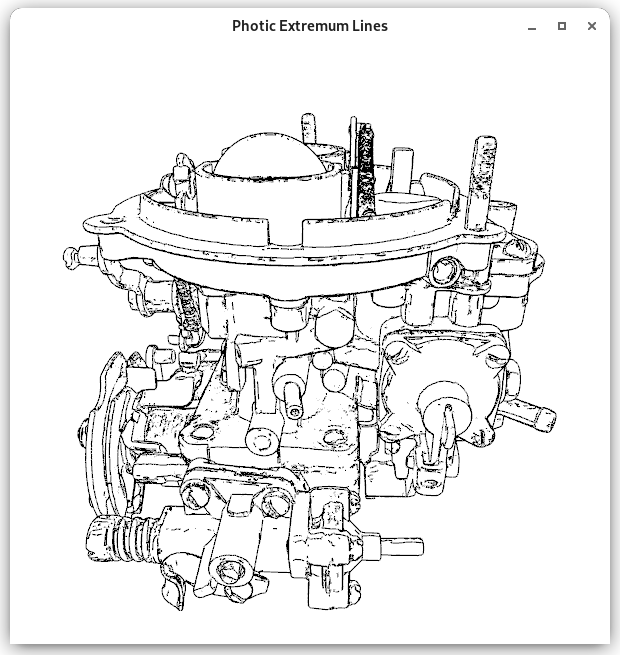
\includegraphics[height=0.49\textheight,trim={15px 15 15 50},clip]{images/tile-contour-pel-shader.png}
    \end{figure}
    \bigskip
    \pause
    \begin{itemize}
      \item<+-> Contours lack details, but are strongest for overall shape
      \item<+-> Photic extremum lines convey additional structure
    \end{itemize}
  \end{frame}

  \begin{frame}{Results: Normal Denoising}
    \begin{minipage}[c]{0.49\textwidth}
      \center
      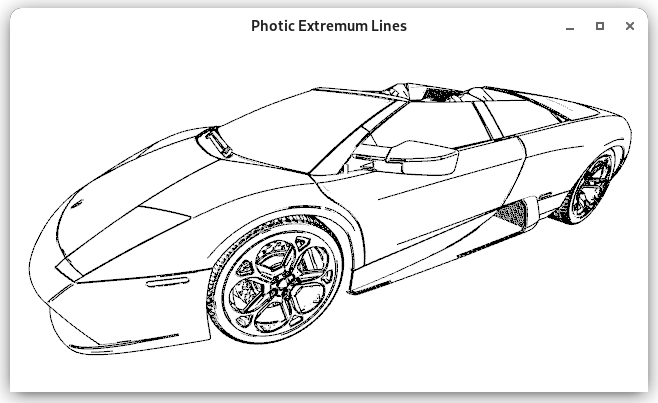
\includegraphics[width=0.8\textwidth,trim={15px 15 15 50},clip]{images/lamborghini-front.png}\\
      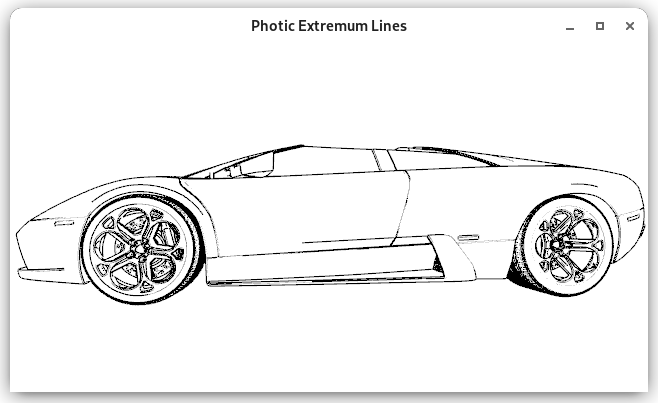
\includegraphics[width=0.8\textwidth,trim={15px 15 15 50},clip]{images/lamborghini-side.png}
    \end{minipage}
    \begin{minipage}[c]{0.49\textwidth}
      \center
      \only<1-3>{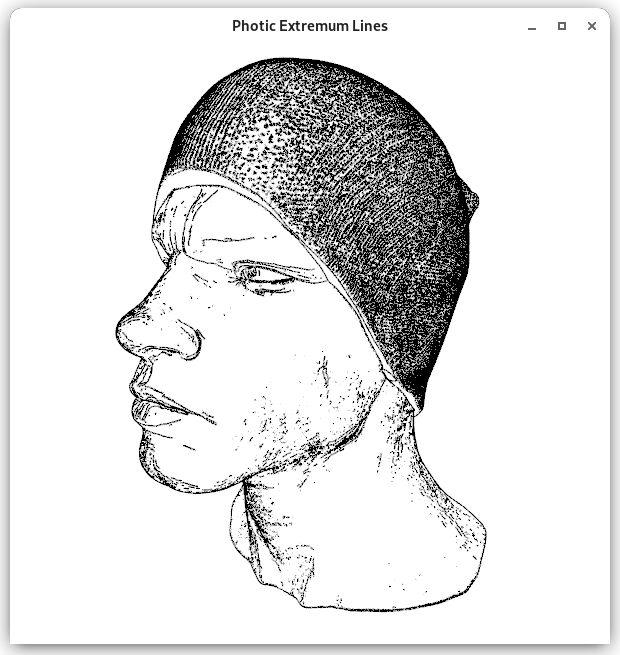
\includegraphics[width=0.8\textwidth,trim={15px 15 15 50},clip]{images/head-contour-pel-shader.png}}%
      \only<4>{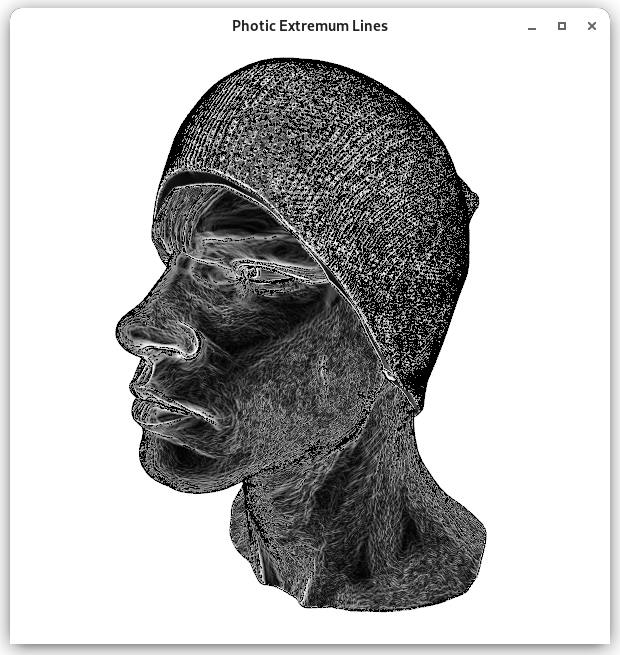
\includegraphics[width=0.8\textwidth,trim={15px 15 15 50},clip]{images/head-light-variation.png}}%
    \end{minipage}
    \pause
    \begin{itemize}
      \item<+-> Scanned models with many triangles often provide noisy normals
      \item<+-> Such noise leads to small feature line artifacts
      \item<+-> Bilateral normal filtering should be applied
    \end{itemize}
  \end{frame}

\section{Conclusions}
  \begin{frame}{Conclusions}
    \textbf{Summary}
    \pause
    \begin{itemize}
      \item<+-> Photic Extremums: $\quad \mathscr{D}_\varphi \norm{\nabla \varphi}(x) = 0\ ,\quad \mathscr{D}_\varphi^2 \norm{\nabla \varphi}(x) < 0$
      \item<+-> View- and light-dependent object-space feature line method
      \item<+-> Computationally expensive third- to fourth-order derivatives
      \item<+-> Convey shapes similar to human perception
    \end{itemize}
    \bigskip
    \pause
    \textbf{Future Work}
    \begin{itemize}
      \item<+-> Faster GPU-based implementation even for volumetric datasets
      \item<+-> Robustness: Exaggerated and mean curvature illumination
      \item<+-> Robustness: Automatic thresholding and noise filtering
    \end{itemize}
  \end{frame}

\begin{frame}
  \vfill
  \centering
  \begin{beamercolorbox}[sep=8pt,center,shadow=true,rounded=true]{title}
    \usebeamerfont{title}%
    Thank you for Your Attention!%
    \par%
  \end{beamercolorbox}
  \vfill
\end{frame}

\begin{frame}
  \frametitle{References}
  % \tiny
  \AtNextBibliography{\tiny}
  \begin{multicols}{2}
    \nocite{decarlo2003}
    \nocite{kolomenkin2008}
    \nocite{rusinkiewicz2006}
    \nocite{meyer2001}
    \nocite{kindlmann2003}
    \printbibliography
  \end{multicols}
\end{frame}

\end{document}
